\label{sec:BSM}
Despite the huge success of the SM, there are many unanswered
questions in the SM which were outlined at the beginning of this chapter. 
Many theories beyond the SM have been developed, which try to include 
the phenomena not explained in the SM and to solve some of the theoretical issues. 
In this section the limitations of the SM theory are summarised and a few BSM
models, considered in this thesis work as they could be observed 
in the \bbtautau\ final state, are introduced.

\subsection{Big questions in the Standard Model}
Some of the important questions unanswered by the SM are outlined in the following:
\begin{itemize}
    \item How to integrate gravity into the SM? 
   Only three fundamental interactions are considered 
in the SM. Attempts to include gravity in the quantum field theory result in 
a theory which is not \textit{renormalisable} (which predicts infinite values for 
observables such as particle masses). Hence gravity is ignored in the SM 
due to its small interaction strength, but that means that the SM will break down 
at large gravitational scales.
    \item What is the nature of dark matter and dark energy?  
Measurement of the cosmic microwave background radiation 
show that the directly observable SM matter is only 5\% of the energy of the universe~\cite{cmb}.
while the dark matter and dark energy makes up about 27\% of the universe and 68\% of the universe,
respectively, where the ratio of dark matter is estimated using measurements 
of galaxy rotation curves~\cite{darkmatter-galaxy} and gravitational lensing~\cite{darkmatter-lense},
and the ratio of dark energy is estimated based on the rate of the universe expansion~\cite{darkenergy}. 
    \item Where does the matter-antimatter assymmetry come from? 
The physical world is made of matter instead of antimatter. 
At the early stage of the universe, the creation and annihilation of the matter-antimatter
was in equilibrium state, but when the universe started to cool down matter and antimatter could only 
annihilate. For matter to survive the annihilation, 
one of the three Sakharov~\cite{Sakharov} condition requires the
\textit{CP-symmetry} to be violated, 
which is the combination of the charge symmetry and the parity symmetry. This phenomenon is observed during 
certain types of weak decay, however the violation in the SM is too small to account for the matter-antimatter
assymmetry.
    \item What is the origin of neutrino masses? 
In the SM, there are no RH neutrinos, and 
there are only Higgs doublets of $\text{SU}(2)_L$, and therefore neutrinos are required to be massless. 
However, observations in neutrino oscillations~\cite{neutrino1, neutrino2} 
imply that the neutrinos have non-zero mass. If neutrinos are normal Dirac 
particles, this will imply an unnaturally small Yukawa coupling to the Higgs field. An other possibility 
to explain its smallness of mass is that neutrinos are \textit{Majorana} particles, 
meaning that neutrinos are their own particles. If this is true, 
processes violating the lepton-number conservation can be allowed, such as the neutrino-less double $\beta$-decay.
    \item Why there are so many free parameters?
As mentioned in section~\ref{sec:SM:intro}, in the SM, there are 26 free parameters 
that have to be input by hand, including the masses of the 12 fermions, the three coupling constants describing the strengths
of the gauge interactions, the two parameters describing the Higgs potential, the eight mixing angles
of the CKM and the \textit{PMNS} (the Pontecorvo-Maki-Nakagawa-Sakata matrix, which accounts for neutrino oscillation) 
matrices, and the CP violation phase in the strong interaction. 
    \item How to solve the \textit{hierarchy problem}? 
The Higgs mass is much smaller than the 
Planck mass $\mathcal{O}$($10^{19}$~GeV). 
The Higgs mass is corrected by quantum loops which are proportional to the square 
of the energy scale, $\Lambda$, and at Planck scale $\Lambda_P\sim10^{19}$~GeV 
these correction becomes very large (if the SM is still valid).
These very large corrections need to be precisely canceled
out to leave the observed Higgs mass of $m_H = 125$~GeV. 
This cancellation requires a high level of fine-tuning and it is therefore considered unnatural,
which is known as the hierarchy problem.
    \item Can the forces be unified? 
In the mid 1970s, it was suggested by Georgi and Glashow that the observed gauge symmetries
of the SM can be accommodated within a larger $\text{SU}(5)$ symmetry group. 
In this Grand Unified Theory (GUT), the coupling constants of the SM are found to 
converge, although not exactly, at the energy scale of about $10^{15}$~GeV.


\end{itemize}

\subsection{Two-Higgs-doublet Model}
\label{sec:BSM:2HDM}
In the SM, the Higgs mechanism assumes a doublet of complex 
scalar fields. While this is the simplest choice, it is not unique. 
The most relavant BSM model to this thesis is the 
two-Higgs-doublet model (2HDM), which is one of the simplest possible extensions of the SM,
first proposed by Tsung-Dao Lee in 1973~\cite{2HDM-李政道}.
He assumed two doublets of complex scalar fields to create a spontaneously CP-violating theory. 
Introducing an additional scalar field might induce flavour-changing neutral currents,
but there are several ways to arrange the yukawa couplings 
so that there is natural flavour conservation~\cite{Weinberg-FCNC}.

Nowadays, there are many motivations for 2HDMs, the best known 
of which might be supersymmetry~\cite{SUSY}. 
The basic idea of supersymmetric theories is that fermions and bosons 
are related to their super-partners which differ in spin by 1/2. 
The introduction of these new particles can solve some of the limitations
in the SM described above, such as the hierarchy problem, force unification and the 
origin of dark matter. 
In supersymmetric theories, the scalars belong to chiral multiplets and  
their complex conjugates belong to multiplets of the opposite chirality; 
since multiplets of different chiralities cannot couple together in the Lagrangian, a
single Higgs doublet is unable to give mass simultaneously to the charge 2/3 and charge
-1/3 quarks. Therefore, an additional doublet is required. 

With some simplifying assumptions, the potential of the two Higgs doublet $\Phi_1$ and
$\Phi_2$ with hyper charge +1 can be written as~\cite{2HDM-Branco}:
\begin{align*}
    V = & m_{11}^2  \Phi_1^\dagger \Phi_1  + m_{22}^2 \Phi_2^\dagger \Phi_2 - m_{12}^2 (\Phi_1^\dagger \Phi_2 + \Phi_2^\dagger \Phi_1) + \frac{\lambda_1}{2}(\Phi_1^\dagger \Phi_1)^2 +\frac{\lambda_2}{2}(\Phi_2^\dagger \Phi_2)^2 \\
    & + \lambda_3 \Phi_1^\dagger \Phi_1 \Phi_2^\dagger \Phi_2 + \lambda_4 \Phi_1^\dagger \Phi_2 \Phi_2^\dagger \Phi_1 +  \frac{\lambda_5}{2}\left[ (\Phi_1^\dagger \Phi_2)^2 + (\Phi_2^\dagger \Phi_1)^2        \right],
\end{align*}
where all parameters are real. 
The vacuum state is then given by:
\[
\Phi_1 =     \begin{pmatrix} 
   0 \\ \ \frac{v_1}{\sqrt{2}} \  \
    \end{pmatrix}, 
\Phi_2 =     \begin{pmatrix} 
    0 \\ \ \frac{v_2}{\sqrt{2}} \  \
        \end{pmatrix}, 
\addtag \]
which give eight fields:
\[
\Phi_a = \begin{pmatrix} 
\phi_a^+ \\ \ (v_a + \rho_a + i \eta_a) /\sqrt{2} \  \
\end{pmatrix}, a = 1,2,    
\addtag \]
where the $\phi_a^+$, $v_a$, $\rho_a$ $\eta_a$ are the four fields
of pertubations around the vacuum state $\Phi_1$ and $\Phi_2$, which makes
a total of eight.  
Three of the eight scalar fields are Goldstone bosons that give mass to the $W$
and the $Z$ bosons, the remaining five fields correspond to five physical Higgs bosons:
two CP-even neutral scalars $h$ and $H_0$, two charged scalar particles $H^\pm$, and a 
CP-odd neutral pseudoscalar $A_0$. 


Like in the single complex field case, the mass terms arise from the square of the field and
the mass terms of the neutral scalars $h$ and $H_0$ can be represented in matrix form as:
\[
\mathcal{L}_{mass}^{ \psi = \rho }   = (\psi_1, \psi_2)\ M(v_1,v_2,\lambda_{1,2,3,4}, m_{12})_\psi\ \begin{pmatrix} 
    \psi_1 \\ \  \psi_2 \ 
    \end{pmatrix},
\addtag \]
where $M(v_1,v_2,\lambda_{1,2,3,4})_\psi$ is the matrix encapsulating the coefficients of the scalar mass terms,
which can be diagonalised by a rotation angle $\alpha$~\cite{2HDM-Branco}.
Similarly for the pseudoscalar $A_0$ and the two charged scalars $H^\pm$,
the mass term is given by:
\[
\mathcal{L}_{mass}^{ \psi = \eta, \phi^\pm }   = (\psi_1^{(+)}, \psi_2^{(+)})\ M(v_1,v_2,\lambda_{4,5}, m_{A,12})_\psi\ \begin{pmatrix} 
    \psi_1^{(-)} \\ \  \psi_2^{(-)} \ 
    \end{pmatrix},
\addtag \]
and the diagonalisation angle is defined as $\tan\beta \equiv \frac{v_2}{v_1}$~\cite{2HDM-Branco}.
% If the doublets are defined as $H_1 = cos \beta \Phi_1 + sin\beta \Phi_2$ and
% $H_2 = -sin \beta \Phi_1 + cos\beta \Phi_2$, the $H_1$ would have a vacuum expectation value 
% of $v/ \sqrt{2} \equiv \frac{(v_1^2+v_2^2)^{1/2}}{\sqrt{2}}$, and $H_2$ has a vacuum expectation value
% of 0.
These two parameters $\alpha$ and $\beta$ determine the interactions of the different Higgs
field with the vector bosons and the fermions (once the Yukawa coupling strength is provided).
In the limit where $\cos(\beta - \alpha) \rightarrow 0$, referred to as `decoupling limit' (or `alignment limit'), 
the lighter neutral scalar $h$ presents almost the same properties as the SM Higgs boson~\cite{decoupling}.
The heavier neutral scalar $H$, on the other hand, could be generated at the LHC which subsequently
decays to two Higgs boson, as shown in the Feynman diagram at leading order in 
Figure~\ref{fig:BSM:resonant}.
Therefore, the resonant di-Higgs production is of interest of this thesis. 
%\usepackage[utf8]{inputenc}
%\usepackage{tikz}
%\usepackage[compat=1.1.0]{tikz-feynman}
%\usepackage{subcaption}
%\usepackage{geometry}

\definecolor{hh_pink}{HTML}{f78fa8}
\definecolor{hh_blue}{HTML}{1e9ee6}
\definecolor{hh_red}{HTML}{ff6900}
\definecolor{hh_med_turq}{HTML}{36B1BF}
\definecolor{hh_lgt_turq}{HTML}{4AD9D9}
\definecolor{hh_whte}{HTML}{E9F1DF}
\definecolor{hh_yllw}{HTML}{FDC536}
%\definecolor{hh_gren}{HTML}{125125}
\definecolor{hh_gren}{HTML}{00CC00}


%\usepackage[EULERGREEK]{sansmath}
%\usepackage{floatrow}
%\DeclareFloatFont{henry}{\sffamily\sansmath}
%\floatsetup[figure]{font=henry}

\begin{figure}[tbh!]
    \centering                      
    \begin{subfigure}[t]{0.5\textwidth}
        \centering
        \begin{tikzpicture}
            \begin{feynman}
                \vertex(g1) at (-3.3, -1.25) {\(\mathbf{g}\)};
                \vertex(g2) at (-3.3, 1.25) {\(\mathbf{g}\)};
                
                \vertex (t1) at (-1.25, -1.25);
                \vertex (t2) at (-1.25, 1.25);
                \vertex (t3) at (0.92, 0);
                
                \vertex (h1) at (2.5, 0);
                \vertex (h2) at (3.7, 1.25) {\(\mathbf{H}\)};
                \vertex (h3) at (3.7, -1.25) {\(\textbf{H}\)};

                \diagram*{
                    (g1) -- [hh_pink,gluon, very thick] (t1),
                    (g2) -- [hh_pink,gluon, very thick] (t2),
                    
                    (t1) -- [hh_red,fermion, very thick] (t2) -- [hh_red,fermion,very thick] (t3) -- [hh_red,fermion,very thick] (t1),
                    
                    (t3) -- [gray,scalar,very thick, edge label'=\(\textbf{X}\)] (h1) -- [hh_blue,scalar,very thick] {(h2), (h3)}
                    
                };
                
            \end{feynman}

        % \filldraw [hh_med_turq] (1.0, 0) circle (3pt);
        % \node[hh_med_turq, scale=1.25] at (1.0, 0.6) {\(c_{tth}\)};
        % \filldraw [hh_pink] (2.5, 0) circle (3pt);
        % \node[hh_pink, scale=1.25] at (2.5, 0.6) {\(c_{hhh}\)};
        
        \end{tikzpicture}
        %\caption{Triangle diagram with $t\bar{t}H$ and $HHH$ couplings}
        \label{fig:SM_diagrams_test:triangle}
        \end{subfigure}%

    \caption[Feynman diagrams, gluon-gluon fusion di-Higgs production]{SM leading-order Feynman diagrams for Higgs boson pair 
    production through resonance of a generic spin-0 scalar particle.}% In SM, $c_{tth}=c_{hhh}=1$ and $c_{tthh}=c_{ghh}=c_{gghh}=0$.}
    \label{fig:BSM:resonant}
\end{figure}

% The most serious potential problem facing all 2HDMs is the possibility of tree level
% flavour-changing neutral currents, which can casue severe phenomenological difficulties.
% Different solutions have been introduced to avoid this problem,
% models which introduce new discrete symmetries to forbid 
% flavour-changing neutral current
% are categorised into type I and type II; 
% models which allow flavour-changing neutral current but suppressed it by making the neutral 
% scalars extremely heavy are categorised in to type III. 
% Type I and type II differ in the how the quarks couple to the two doublets, where in
% the type I only one doublet couples to the quarks and in the type II one doublet couples to 
% one type of quark (up or down type).
In chapter~\ref{sec:search for dihiggs}, searches for the di-Higgs production from resonance 
of a generic heavy spin-0 neutral scalar is presented. The resonance particle is assumed to have a narrow
decay width, and the normalisation of resonant production in the analysis is set to 
\[
\sigma \times BR_{\bbtautau}  = \SI{1}{pb} \times 0.073  =  \SI{0.073}{pb},
\addtag \]
where dummy cross-section of 1 pb is chosen for the resonant production.
% to make combination with other decay channels easier, 
% and to ease scaling of the signal 
% for the calculation of the cross-section limits 
% (more details in Section \ref{sec:DiHiggs:results}).
% The search is therefore very relavant to the heavier scalar $H_0$.
% Since the 2HDMs provide two neutral CP-even scalars, $h$ and $H_0$, where the lighter
% $h$ presents almost the same properties as the SM Higgs boson.

\subsection{Effective field theory interpretation}
% Take an example of a cow, which is a complicated system with multiple stomachs made of cells
% made of proteins made of atoms and so on. A `cow-cow' scattering problem might 
% be an extremely difficult task to tackle. However, if one views from far enough away, 
% the two cows scattering behave point-like, and the problem becomes a matter of simple 
% interaction.
% Using the similar philosophy, 
% The basic idea of effective field theories (EFTs)
% is to approximate a physical system by integrating out the degrees of
% freedom that are not relevant in a given experimental setting. 
Instead of a \textit{theory of everything}, 
physicists' focus these days is on less ambitious 
but more practical \textit{theories of something}, which describe particular physical
systems in particular conditions. Such theories are seen as effective fields theories (EFTs)
because they are not meant to be valid at all energy scales, and often the degrees of
freedom they describe are emergent rather than fundamental.

The basic idea behind EFTs is that things simplify when viewed from a distance.
% Take an example of a cow, which is a complicated system with multiple stomachs made of cells
% made of proteins made of atoms and on and on. A `cow-cow' scattering problem might 
% be an extremely difficult task to tackle with using QED and QCD. 
% However, if one views from far enough away, the internal structure of the cows can be ignored, 
% and the problem reduces to a simple elastic interaction.
% There is nothing new in an EFT, that it includes all effects relevant 
% at a given scale, but not those that only play a role at significantly 
% different scales.  
In particle physics, `viewing from far away' is equivalently saying that the energy
scale being considered is low. 
The SM is commonly accpeted as an effective theory applicable 
up to energies not exceeding a certain scale $\Lambda$. 
For a field theory valid above that scale, it needs to satisfy a few requirements:
\begin{itemize}
    \item it should have a gauge group that contains the SM $\text{SU}(3)_C \times \text{SU}(2)_L\times \text{U}(1)_Y$ group,
    \item it should incorporate all degrees of freedom of the SM,
    \item it should reduce to the SM at low energies.
\end{itemize}
In most cases, the reduction to the SM is achieved by 
decoupling the heavy particles with masses of order $\Lambda$ or larger. 
If one writes down the Lagrangian of a BSM theory, 
the BSM part will be suppressed by powers of $\Lambda$:
\[  
    \mathcal{L}_{BSM} = \mathcal{L}^{(4)}_{SM} + \frac{1}{\Lambda} \sum_k c^{(5)}_k O^{(5)}_k+
    \frac{1}{\Lambda^2} \sum_k c^{(6)}_k O^{(6)}_k + \mathcal{O} \left(\frac{1}{\Lambda^3}\right),
\addtag \]
where $\mathcal{L}^{(4)}_{SM}$ is the SM Lagrangian which contains dimension-two
and -four operators only, and the BSM physics is encapsulated by operators of 
dimension-five, dimension-six $O^{(5)}_k$, $O^{(6)}_k$ 
and of higher dimensions (suppressed by higher order of $\Lambda$)~\cite{EFT}.
The $c^{(n)}_k$ are the dimensionless coupling constants (\textit{Wilson coefficients}).

It has been proven in Ref.~\cite{EFT} that the dimension-five operator
(insterstingly, there is only one of such operator) violates 
the lepton number conservation, while at the LHC this effect is almost
unobservable, therefore it is not considered.
On the other hand, it is possible to write down a large number of dimension-6 operators, 
for example, just attaching an extra term $\phi^\dagger\phi$
to any of the terms in the SM Lagrangian will
be dimension-six. It was shown in Ref.~\cite{EFT-dimension-6} there are 59 of them.
Some BSM operators have the effect of rescaling the Higgs boson coupling to other 
particles, and some create new anomalous couplings which were not allowed in the SM. 
In both scenarios the di-Higgs production receives corrections on the production
cross-section, in some cases the cross-section is greatly enhanced, making 
the observation of di-Higgs possible with current LHC data.

One major benefit of the EFT approach is that it is `model independent'.
Same set of low energy operators (the ones of the SM) can be reused for different 
BSM theories, in contrast to the `model dependent' approach, 
where one searches for the signatures of a specific new particle(s). 

There are two approaches to treating the SM as an EFT:
Standard Model EFT (SM EFT)~\cite{EFT-dimension-6} and Higgs EFT (HEFT)~\cite{HEFT1, HEFT2}.
The SM EFT in general is a simpler framework due to more restrictive symmetries:
the operators follow the $\text{SU}(3)_C \times \text{SU}(2)_L\times \text{U}(1)_Y$ gauge symmetry.
On the other hand, the only manifest gauge symmetry of 
HEFT is $\text{SU}(3)_C \times \text{U}(1)_{\text{em}}$,
while the  $\text{SU}(2)_L\times \text{U}(1)_Y$ symmetry is non-linearly realised.
In this formalism, anomalous Higgs boson couplings are expected to be the 
dominant effects on new physics in the electroweak sector. 
Deviations from SM predictions can potentially be observed via 
di-Higgs production using the HEFT framework.
% In particular, EFTs ignore spatial substructures much 
% smaller than the lengths of interest, or effects at much higher energies 
% than the energy scale of interest~\cite{EFT}.

In the HEFT Lagrangian, ggF $HH$ production is described at LO with 
5 operators and their corresponding Wilson coefficients: $c_{hhh}, c_{tth}, c_{tthh}, c_{ggh}$ 
and $c_{gghh}$. 
The first two Wilson coefficients are the couplings modifiers 
of the $HHH$, $ttH$ vertices, 
i.e.\  $c_{hhh} \equiv \kappa_\lambda =  \lambda_{HHH} / \lambda^{\text{SM}}_{HHH}$ and 
$c_{tth}  = \lambda_{ttH} / \lambda^{\text{SM}}_{ttH}$,
with $\lambda_{HHH}$ being the Higgs boson self-coupling constant 
and $\lambda_{ttH}$ being the top-quark Yukawa coupling. 
While these two modifiers are responsible for SM vertices,
the rest accounts for the Non-SM interactions,
affect respectively the $ttHH$, $gHH$ and $ggHH$ vertices. 
The Feynman diagrams for such interactions and the corresponding
Wilson coefficients are shown in Figure~\ref{fig:BSM:HEFT_diagrams}.
The HEFT Lagrangian reduces to the SM Lagrangian for $c_{hhh} = c_{tth} = 1$ 
and $c_{tthh} = c_{ggh} = c_{gghh} = 0$, when the Higgs boson self-coupling 
and top-quark Yukawa coupling have SM values 
and none of the BSM production modes are present. 
% therefore the HEFT Lagrangian reduces to the SM Lagrangian.
% when $c_{hhh} =c_{tth} = 1$ and $c_{tthh} = c_{ggh} = c_{gghh} = 0$.
%The three non-SM LO Feynman diagrams for $HH$ production through gluon-gluon fusion, introduced in HEFT, are described by the Feynman diagrams shown in \Fig{\ref{fig:HEFT_diagrams_o6}}.
%The HEFT formalism allows us to make a more general measurement of the Higgs self-coupling and explore different BSM scenarios by simultaneously varying multiple Wilson coefficients \cite{Cohen:2020xca}.

Higgs boson pair production is the most promising process to measure the 
Higgs boson self-coupling because it gives access to $c_{hhh}$ at tree level.
Furthermore the \HH process gives unique access to 
the two other Wilson coefficients, $c_{tthh}$ and $c_{gghh}$.
% On the contrary, single Higgs boson processes have better sensitivity to the remaining two coefficients, $c_{tth}$ and $c_{ggh}$.
The HEFT formalism allows us to interpret general searches in different BSM scenarios 
by simultaneously varying multiple Wilson coefficients. 
%\usepackage[utf8]{inputenc}
%\usepackage{tikz}
%\usepackage[compat=1.1.0]{tikz-feynman}
%\usepackage{subcaption}
%\usepackage{geometry}

\definecolor{hh_pink}{HTML}{f78fa8}
\definecolor{hh_blue}{HTML}{1e9ee6}
\definecolor{hh_red}{HTML}{ff6900}
\definecolor{hh_med_turq}{HTML}{36B1BF}
\definecolor{hh_lgt_turq}{HTML}{4AD9D9}
\definecolor{hh_whte}{HTML}{E9F1DF}
\definecolor{hh_yllw}{HTML}{FDC536}
%\definecolor{hh_gren}{HTML}{125125}
\definecolor{hh_gren}{HTML}{00CC00}

%\usepackage[EULERGREEK]{sansmath}
%\usepackage{floatrow}
%\DeclareFloatFont{henry}{\sffamily\sansmath}
%\floatsetup[figure]{font=henry}

\begin{figure}[tbh!]
    \centering                          
    \begin{subfigure}[t]{0.3\textwidth}
        \centering
        \begin{tikzpicture}
               \begin{feynman}
                
                \vertex(g1) at (-2.3, -1.3) {\(\mathbf{g}\)};
                \vertex(g2) at (-2.3, 1.3) {\(\mathbf{g}\)};
                \vertex (ggh) at (-0.8, 0);
                \vertex (h1) at (0.8, 0);
                \vertex (h2) at (2.2, 1.3) {\(\mathbf{H}\)};
                \vertex (h3) at (2.2, -1.3) {\(\textbf{H}\)};

                \diagram*{
                    (g1) -- [color=hh_pink, gluon,very thick] (ggh),
                    (g2) -- [color=hh_pink, gluon,very thick] (ggh),
                    (ggh) -- [color=hh_blue, scalar, very thick] (h1) -- [color=hh_blue, scalar, very thick] {(h2), (h3)}
                };
                
            \end{feynman}

        \filldraw [black] (-0.8, 0) circle (2pt);
        \node[ scale=1.25] at (-0.8, 0.6) {\(c_{ggh}\)};
        \filldraw [black] (0.8, 0) circle (2pt);
        \node[scale=1.25] at (0.8, 0.6) {\(c_{hhh}\)};
        \node[scale=1] at (0.0, -0.6) {\(\textbf{H}\)};
        
        \end{tikzpicture}
    \caption{ggh and hhh}
    \end{subfigure}
    \begin{subfigure}[t]{0.3\textwidth}
        \centering
        \begin{tikzpicture}
            \begin{feynman}

		\vertex(g1) at (-1.6, -1.3) {\(\mathbf{g}\)};
                \vertex(g2) at (-1.6, 1.3) {\(\mathbf{g}\)};
                \vertex (t) at (0.0, 0);
		\vertex (h1) at (1.6, 1.3) {\(\mathbf{H}\)};
                \vertex (h2) at (1.6, -1.3) {\(\textbf{H}\)};

                \diagram*{
                    (g1) -- [color=hh_pink, gluon,very thick] (t),
                    (g2) -- [color=hh_pink, gluon,very thick] (t),
                    (t) -- [color=hh_blue, scalar, very thick] {(h1), (h2)}

		};

            \end{feynman}

        \filldraw [black] (0.0, 0.0) circle (2pt);
        \node[ scale=1.25] at (0.0, 0.6) {\(c_{gghh}\)};

        \end{tikzpicture}
    \caption{gghh}
    \end{subfigure}
    \begin{subfigure}[t]{0.3\textwidth}
        \centering
        \begin{tikzpicture}
            \begin{feynman}

                \vertex(g1) at (-2.5, -1.25) {\(\mathbf{g}\)};
                \vertex(g2) at (-2.5, 1.25) {\(\mathbf{g}\)};

                \vertex (t1) at (-1.0, -1.25);
                \vertex (t2) at (-1.0, 1.25);
                \vertex (t3) at (0.5, 0);

                \vertex (h1) at (2.0, 1.25) {\(\mathbf{H}\)};
                \vertex (h2) at (2.0, -1.25) {\(\textbf{H}\)};

                \diagram*{
                    (g1) -- [color=hh_pink, gluon,very thick] (t1),
                    (g2) -- [color=hh_pink, gluon,very thick] (t2),

                    (t1) -- [color=hh_red, fermion,very thick] (t2) -- [color=hh_red, fermion,very thick] (t3) -- [color=hh_red, fermion,very thick] (t1),

                    (t3) -- [color=hh_blue, scalar, very thick] {(h1), (h2)}

                };

            \end{feynman}

        \filldraw [black] (0.55, 0) circle (2pt);
        \node[scale=1.25] at (0.55, 0.6) {\(c_{tthh}\)};

        \end{tikzpicture}
    \caption{tthh}
    \end{subfigure} \\                                                                                                                                                                                     

    \caption[Feynman diagrams, gluon-gluon fusion di-Higgs production]{BSM HEFT leading order Feynman diagrams for Higgs boson pair production through gluon-gluon fusion.}% In SM, $c_{tth}=c_{hhh}=1$ and $c_{tthh}=c_{ghh}=c_{gghh}=0$.}
    \label{fig:BSM:HEFT_diagrams}
\end{figure}






% EFT gives a practical and simplified description of a full or underlying theory, 
% which by assumption, is correct at all energy scales. 
% To build a EFT, one needs to specify an energy scale $\Lambda$, 
% that the EFT can correctly describes the physics happends at energy scales $E << \Lambda$, 
% with some finite precision. 
% This scale hierarchy between the energy of interest and
% the scale of high-energy physics not included in the EFT is the basic requirement for the
% EFT idea. 

% Linking the idea of EFT to the Higgs sector and the LHC, 
% one may be interested in asking a question: 
% what is the best language to discuss indirect signs of new physics,
% at the scale of the LHC can reach?
% Given the large number of BSM models and possible physics observables, 
% it would be highly impractical to interpret the experimental measurements 
% using the complete model. Instead it would be much more convenient to use the 
% EFT method to define an intermediate framework that can be linked to the 
% complete model and the measurements. 
% By dimensional analysis, one can see that the SM Lagrangian has a \textit{mass dimension}
% of 4. One can then write the BSM Lagrangian by appending the Lagrangian of the SM 
% by BSM operators of mass dimension 6, i.e.\ 
% \[
% \mathcal{L}_{EFT} = \mathcal{L}_{SM} + \sum_i \frac{f_i}{\Lambda^2}\mathcal{O}_i,
% \addtag \]
% where $\mathcal{O}_i$ is some BSM operators of dimension 6, $\Lambda$ is the cutoff energy, and
% $f_i$ are the \textit{Wilson coefficients} that are dimensionless constant and
% encapsulate the coupling strength.
% It is possible to write down a large number of dimension-6 operators, 
% for example, just attaching an extra term $\phi^\dagger\phi$
% to any of the terms in the SM Lagrangian will
% be dimension-6. It was shown in Ref.~\cite{EFT-dimension-6} there are 59 of them.
% Some BSM operators have the effect of rescaling the Higgs boson coupling to other 
% particles, and some create new vertices which were not allowed in the SM, and ultimately
% changing the cross-section of the di-Higgs production which is the main interest of 
% this thesis. 

Linking the idea to the non-resonant di-Higgs production modes as shown in Figure~\ref{fig:SM:di-Higgs-ggf},
where the Box diagram amplitude is proportional to the square of the top
yukawa coupling, $g_t^2 = \kappa_t^2$ and the triangle amplitude is 
proportional to the square of $g_t g_{HHH} = \kappa_t \kappa_\lambda$,
the destructive amplitude can be written as 
(and if one does not consider additional anomalous couplings):
\[
A(\kappa_t, \kappa_\lambda)  = \kappa_t^2 B +  \kappa_\lambda^2  T,
\addtag \]
where A is the amplitude of the ggF $HH$ production and the 
$B$ and $T$ are the contribution from the box and triangle diagram, respectively. 
Due to the BSM operators, the coupling $\kappa_t$, $\kappa_\lambda$ can be rescaled.
Taking the square of the amplitude, the cross-section is approximately:
\[
\sigma \sim \kappa_t^4 \left(  |B|^2 + \frac{\kappa_\lambda}{\kappa_t} (BT +TB) + (\frac{\kappa_\lambda}{\kappa_t})^2 |T|^2  \right),    
\addtag \]
which is a function of only the $\kappa_t$ and $\frac{\kappa_\lambda}{\kappa_t}$.
While the cross-section is determined by both of them, if one sets the 
$\kappa_t$ equals to 1 (which is the SM case), the kinematics is only 
determined by the $k_\lambda$.
An example of this dependency is shown in Figure~\ref{fig:BSM:kl_mhh}
Using this feature, one can perform a scan of possible $k_\lambda$ values,
excluding values of $k_\lambda$ that have incompatible kinematics with the 
experimental data. 
Such a scan is presented in chapter~\ref{sec:search for dihiggs},
where the ggF and VBF di-Higgs non-resonant production process are assumed to have 
various $k_\lambda$ values, and the kinematics distributions are compared
with the data using Multivariate techniques for compatibility.

\begin{figure}[htbp]
\centering
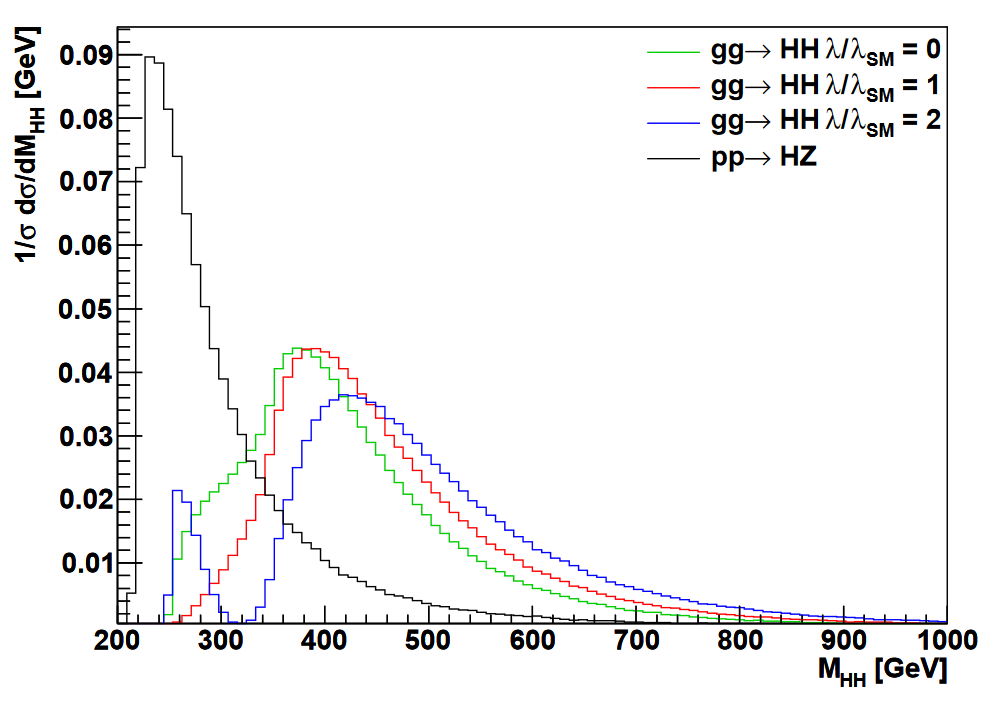
\includegraphics[width=.41\textwidth]{theory/plots/kl_mhh.png}
\caption{An example of mass of the di-Higgs system distribution, 
varying for different values of $k_\lambda$ along with a typical
background $pp \rightarrow ZH$. Image taken from Ref.\cite{kl_mhh}.
}
\label{fig:BSM:kl_mhh}
\end{figure}